\documentclass[12pt,a4paper]{article}

\usepackage{alltt}
\usepackage[utf8]{inputenc}
\usepackage[english]{babel}
\usepackage{amsmath}
\usepackage{amsfonts}
\usepackage{amssymb}
\usepackage{indentfirst}
\usepackage{setspace}
\usepackage[pdftex]{graphicx}
\usepackage{caption}
\usepackage{subcaption}
\usepackage{textcomp}
\usepackage{array}
\usepackage{listings}
\usepackage{color}
\usepackage{tikz} % для создания иллюстраций
\usepackage{hyperref}

\newcommand{\infers}{\,\to\,}
\newcommand{\tinfers}{\;\Rightarrow\;}

%\voffset = -118pt
%\textheight = 820pt
%\hoffset = -100pt
%\textwidth = 550pt
\newcommand{\htext}{0.46\textwidth}
\newcommand{\hstext}{0.45\textwidth}

\newcommand{\mat}[1]{\overline{#1}}
\newcommand{\framed}[1]{\tikz[baseline=(char.base)]{\node[shape=rectangle,draw,inner sep=4pt] (char) {#1};}}

%opening
\title{}
\author{}

\begin{document}


% TEAM.
\parbox{0.333\textwidth}{
	Maksim Velikanov \\[0mm]
}
% In der Mitte der Name der Veranstaltung.
\parbox{0.333\textwidth}{\vspace*{1mm}\begin{center}\large\bf%
		HPC with C++\\[0mm]
		SS 24\\[0mm]
\end{center}}
\parbox{0.333\textwidth}{
	\begin{flushright}
		Project report\\[0mm]
		17.02.2025\\[0mm]
	\end{flushright}
}
\par\vspace{-5mm}
\definecolor{freiburg-gray}{rgb}{0.68,0.68,0.68}
\vspace*{2mm}
\raisebox{1.19cm}{%
	\textcolor{freiburg-gray}{\rule{\textwidth}{1.1mm}}}

\bigskip




\section{Introduction}

The implemented program is capable of generating a cubic lattice or using a precomputed one; running the simulation under control without the cluster vaporizing; monitoring the energies; saving the cluster for visualization; heating the cluster and measuring the melting point and latent heat; running parallel simulation with OpenMPI; stretching a golden whisker and measuring stress.

The theoretical base is present in \hyperref[methods]{methods}, the overview of implementation and results in \hyperref[implementation]{implementation}, and \hyperref[conclusion]{conclusion} at the end.

\section{Methods}
\label{methods}

The key components of Molecular Dynamics are following:

\begin{enumerate}
	\item Update atom position and velocity, given constant force for a small time step --- {\bf Velocity-Verlet integrator}
	\item Estimate force between particles from the potential energy --- {\bf Lennard-Jones potential}
	\item Prevent explosion of the system by connecting it to a constant-temperature heat bath --- {\bf Berendsen Thermostat}
	\item More accurate N-body potential for modeling metals --- {\bf Embedded Atom Method potential}
	\item {\bf Domain decomposition} and parallel execution with OpenMPI
	\item Application of an external force --- {\bf Stress estimation}
\end{enumerate}

\newpage
\subsection*{Velocity-Verlet integrator}

The movement is approximated by assuming constant force and making small time steps. We take Newton's law and definition of velocity, using Taylor formula, we get the approximation equations. Was rediscovered by Loup Verlet \cite{verlet} for Molecular Dynamics simulation.

\[ \dot{\mat{v}}_i(t) = \cfrac{\mat{f}_i(t)}{m_i} \]
\[ \dot{\mat{r}}_i(t) = \mat{v}_i(t) \]

Integration, predictor step:
\[
v_i(t + \Delta t/2) = v_i(t) + \cfrac{1}{2m_i} f_i(t) \Delta t
\]
\[ r_i(t+\Delta t) = r_i(t) + v_i(t+ \Delta t/2) \Delta t \]

Corrector step:
\[ v_i(t+\Delta t) = v_i(t+\Delta t/2) + \cfrac{1}{2m_i}f_i(t+\Delta t) \Delta t \]

{\bf Implementation} --- src/atoms.h, src/verlet.cpp, src/verlet.h, tests/test\_verlet.cpp

\subsection*{Lennard Jones potential}

Here we derive a formula to compute the force from potential energy. By definition of pair potential:
\[
E_{pot} = \sum_{i<j} V(r_{ij})
\]

Lennard-Jones potential \cite{lennard-jones} is sum of Pauli Repulsion (repulsive force) and London Dispersion (attractive force). These interactions act even on uncharged atoms.

\[
V_{ij}(r) = 4\epsilon \left( \Bigl(\cfrac{\sigma}{r}\Bigr)^{12} - \Bigl(\cfrac{\sigma}{r}\Bigr)^{6} \right)
\]

By definition of energy, force is the derivative of energy by position.
\[
\mat{f}_k = \left( \begin{aligned}
	& - \partial E / \partial x_k \\
	& - \partial E / \partial y_k \\
	& - \partial E / \partial z_k \\
\end{aligned} \right) = \sum_i \cfrac{\partial V}{\partial r_{ik}} {\hat r_{ik}} \text{\ (unit vector)}
\]

Let's compute for one of the dimensions.
\[
\cfrac{\partial V_{ij}}{\partial x_k} = \text{(chain rule by vector length)} \cfrac{\partial V_{ij}}{\partial r_{ij}} \cfrac{\partial r_{ij}}{\partial x_k}
\]

\[ \cfrac{\partial r_{ij}}{\partial x_k} = \cfrac{\partial \sqrt{(x_j-x_i)^2 + \ldots}}{\partial x_k} = (*) \]
Remember: \( (\sqrt{u})' = \cfrac{1}{2\sqrt{u}} u' \)

\[
(*) = \cfrac{1}{2r_{ij}} \cfrac{(x_j-x_i)^2+\ldots}{\partial x_k} = \cfrac{1}{r_{ij}} \cdot (x_j-x_i) \cdot \Bigl(\cfrac{\partial x_j}{\partial x_k} - \cfrac{\partial x_i}{\partial x_k}\Bigr)
\]
Here is a pair of atoms $i$ and $j$. We want the force for atom $k$. If \(k\neq i\) and \(k\neq j\), the expression is 0.

\[
(*) = \left( \begin{aligned}
	& (x_j - x_i) (\delta_{jk} - \delta_{ik}) / r_{ij} \\
	& (y_j - y_i) (\delta_{ik} - \delta_{jk}) / r_{ij} \\
	& (z_j - z_i) (\delta_{ik} - \delta_{jk}) / r_{ij} \\
\end{aligned} \right) 
\]

\[
k=j \infers (x_k-x_i)(1-0)/r_{ik},\ (*) = {\hat r_{ik}}
\]
\[
k=i \infers (x_j-x_k)(0-1)/r_{kj},\ (*) = {\hat r_{jk}}
\]

When we take the derivative of energy, only the pairs, where one of the atoms is \(k\), are left. The derivative is exactly the same for \(V_{ij}\) and \(V_{ji}\).

{\centering\framed{ \( \mat{f}_k = - \sum_i \cfrac{\partial V}{\partial r} {\hat r_{ik}} \) }\\}

Last piece in the puzzle is derivative of potential by distance.

\[
\cfrac{\partial V}{\partial r} = 4\epsilon (\sigma^{12} (-12) r^{-13} - \sigma^6\cdot 6\cdot r^{-7})
\]

\subsection*{Berendsen thermostat}

As the molecular dynamics system evolves, potential energy decreases and kinetic energy increases. Kinetic energy is temperature multiplied by a constant: $E_k = \frac{3}{2} NK_b T$, so the temperature can get too high and system will explode. Therefore we connect the system to a heat bath of constant temperature, which stabilizes the simulation. The Berendsen thermostat \cite{berendsen} decreases the temperature by scaling the velocities of atoms by a factor:

\[ v' = \lambda v \]

\[ \lambda = \sqrt{1 + \left(\cfrac{T_0}{T}-1 \right) \cfrac{\Delta t}{\tau} }  \]
\[ E_k = \cfrac{1}{2} \sum_i m_i v_i^2 = \cfrac{3}{2} N K_b T \infers T = \cfrac{2}{3} \cfrac{E_k}{K_b N} \]

\(T_0\) is target temperature, \(\Delta t = 0.0001 \sqrt{m\sigma^2 / \epsilon} \) from the first simulation, \( \tau \) is relaxation time of the thermostat and should be much larger than the time step.

\subsection*{Embedded Atom Method potential}

TODO cite Cleri Rosato

The EAM models attraction with the local electron density, and repulsion with a pairwise term. This potential has parameters that must be estimated for each type of atom experimentally, in this report we use gold (Au).

Force is the derivative of energy by position:
\[
\mat{f}_k = -\cfrac{\partial E_{pot}}{\partial \mat{r}_k}
\]

\[
\mat{f}_k = \sum_i ( \partial F(\rho_k) / \partial \rho_k + \partial F(\rho_i) / \partial \rho_i )  \cfrac{\partial f}{\partial r_{ik}} \hat{r}_{ik} +
\sum_i \cfrac{\partial V}{\partial r_{ik}} \hat{r}_{ik},
\]

where $\mat{f}_k$ is force on atom $k$, $r_k$ is position of atom $k$, $F(\rho)$ is an embedding functional dependent on electron density, $V$ is pairwise repulsion.

\subsection*{EAM potential, time and mass units}

We fix the length to angstrem (approximately distance between atoms) and energy to electron-volts (energy of a covalent bond) at first:

\begin{itemize}
	\item length: Å, angstrem = 0,1nm. 1m = $10^{10}$ Å
	\item energy: eV, electron-volts = qU Joules = 1 (elementary electrical charge) $* 1,602 * 10^{-19}$ Volts. 1 Joule = $\frac{1}{1U}$
	\item velocity: $[l]/[t]$
	\item acceleration: $[l]/[t]^2$
	\item $f=ma$:       $[m][l]/[t]^2$
	\item $[E]=[A]=[f*S]$:    $[m][l]^2/[t]^2$
	\item $f$: $[E]/[l]$
\end{itemize}

Boltzmann constant in new unit system: \[ K_b = 1,38 * 10^{-23} \frac{J}{K} = \frac{1,38}{1,602} * 10^{-23} * 10^{+19} \text{eV/K} = 0,8614 * 10^{-4} = \underline{8,614 * 10^{-5} \text{eV/K}} \]

We fix \underline{[t] = 1 fs}. From this derive the unit of mass: 

\begin{gather*}
	[E] = [m][l]^2/[t]^2\\
	[m] = [E][t]^2/[l]^2\\
	[m] = 1 \text{eV} * (1 \text{fs})^2 / (1 \text{Å}^2) =\\
	1,602 * 10^{-19} J * 10^{-30} s * 10^{+20} m = 1,6 * 10^{-29} \text{kg}
\end{gather*}

We can convert this to g/mol:
\begin{center}
	1mol $= 6.02 * 10^{23}$\\
	1 g/mol = $\cfrac{10^{-3}}{6 * 10^{23}} $\\
	1 kg = $6 * 10^{26}$ g/mol\\
	$[m] = 1,6 * 10^{-29} * 6 * 10^{+26} \text{g/mol} = 9,6 * 10^{-3} =$ \underline{0,009649 g/mol}\\
	1 g/mol = $103,63\ [m]$
\end{center}

Now 1 gold atom has mass 196,96 * 103,63 $[m]$.

\subsection*{Domain decomposition}

We fix the region of simulation and divide it into a regular grid. Size of the region is $[0, L_x] \times [0, L_y] \times [0, L_z]$, for each dimension we divide it into $N_x, N_y, N_z$ subdomains. We spawn the same amount of parallel processes as there are subdomains. Each process holds all atoms in its subdomain and the atoms near the border of subdomain (ghost atoms) not further than $2 * cutoff$ for EAM potential.

The processes have to communicate the atom movement between subdomains and ghost atoms with the neighboring subdomains. Each subdomain has $9+8+9=26$ neighbors in 3D. To avoid pair-wise communication between them, we execute send-receive (Fig.~\ref{fig:domain-communication}):

\begin{enumerate}
	\item in $x+$ direction
	\item in $x-$ direction
	\item in $y+$ direction
	\item in $y-$ direction
	\item in $z+$ direction
	\item in $z-$ direction
\end{enumerate}

\begin{figure*}[h!]
	\centering
	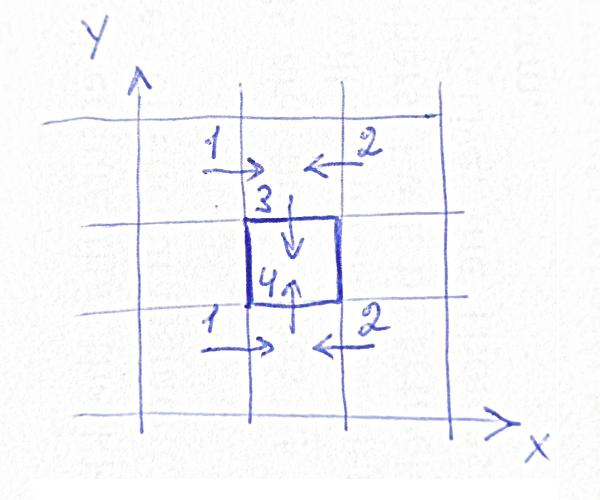
\includegraphics[width=.5\linewidth]{img/milestone08-domain-communication.jpg}
	\caption{Each process gets neighbor information without direct communication.}
	\label{fig:domain-communication}
\end{figure*}

This way it takes 6 steps instead of 26 for each process to get all information from its neighbors.

\subsection*{Stress estimation}

For the experiment with stretching a golden whisker we need to compute the reaction to strain --- the stress matrix.

\[
\sigma = \cfrac{1}{V} \sum_{i<j} \mat{r}^T_{ij} \times \mat{f}_{ij} = \cfrac{1}{V} \sum_i^{N} \sum_{j=i}^{N+N_G} \mat{r}^T_{ij} \times \mat{f}_{ij},
\]

where $\sigma\ (3, 3)$ - stress matrix for $xx, xy, \ldots zz$ directions, $V$ - total volume, $\mat{r}^T_{ij}\ (1, 3)$ - position, $\mat{f}_{ij}\ (3, 1)$ - force.

As we stretch the whisker in the $Z$ axis, I take only $\sigma(3, 3)$ value from this matrix (in experiments all other entries are near 0). The stress is per-atom, can be computed separately in each subdomain and then summed.



\clearpage

\section{Implementation and results}
\label{implementation}

Note! Copying .xyz files in Meson didn't work for me, so I had to copy them to build directory by hand.

Code is structured in folders:
\begin{itemize}
	\item milestones --- CPP sources for simulation executables
	\item plot --- Python notebooks for plotting. Requires precomputed simultion results
	\item report --- the sources for the report you are reading now
	\item src --- common CPP files
	\item tests --- CPP tests using Google test framework
\end{itemize}

\subsection*{First simulation}
In the first simulation, we don't care about physical units, and just set \( m=1, \sigma=1, \epsilon=1 \). Simulation duration is \( 100 \sqrt{m\sigma^2 / \epsilon} \), the atom positions are saved each \( 1 \sqrt{m\sigma^2 / \epsilon} \).  

Experimentally choosing the time step (multiplied by \( \sqrt{m\sigma^2 / \epsilon} \)): 0.001 --- OVITO visualization shows that most of atoms evaporate and fly into infinity; 0.00001 --- most atoms stay together, while some still evaporate. We can also detect evaporation if potential energy increases and kinetic energy doesn't change. The total energy was plotted for different time steps in Fig.~\ref{fig:first_simulation}.

{\bf Implementation} --- src/lj\_direct\_summation.cpp, src/lj\_direct\_summation.h, tests/test\_lj\_direct\_summation.cpp, src/xyz.cpp, src/xyz.h, tests/test\_verlet.cpp, milestones/04/main.cpp

\begin{figure*}[htb]
	\centering
	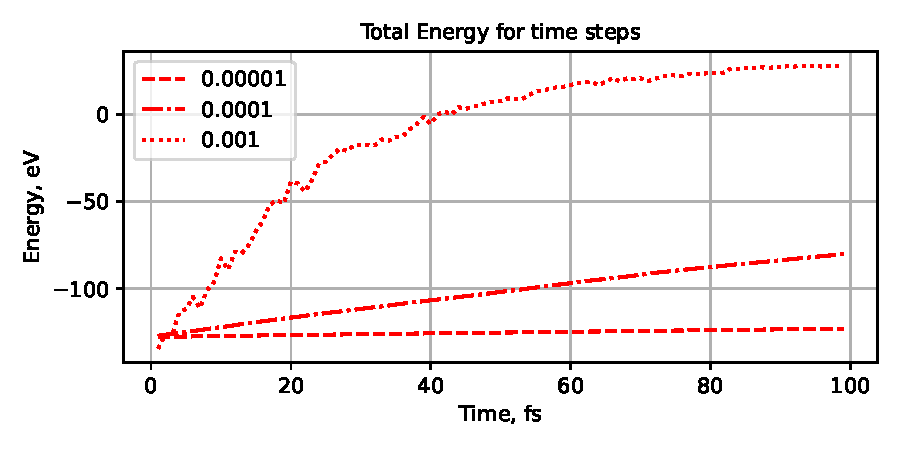
\includegraphics[width=.7\linewidth]{img/fig_total_energy.pdf}
	\caption{Less atoms evaporate with very small time step.}
	\label{fig:first_simulation}
\end{figure*}


\subsection*{Berendsen thermostat}

\begin{figure*}[htb]
	\centering
	\begin{minipage}{.3\textwidth}
		\centering
		\resizebox{\columnwidth}{!}{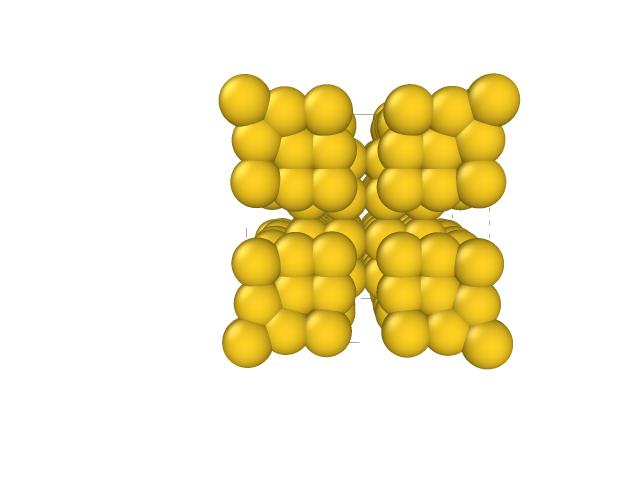
\includegraphics[trim={1.8cm 1.8cm 2.2cm 1.8cm},clip]{img/sim1.jpg}}
	\end{minipage}\hfill
	\begin{minipage}{.3\textwidth}
		\centering
		\resizebox{\columnwidth}{!}{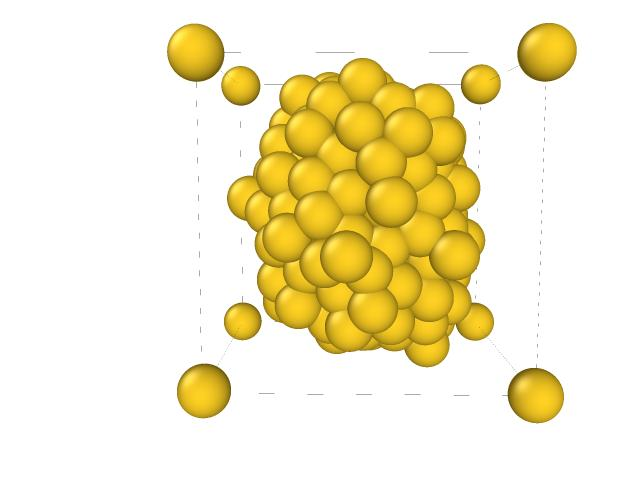
\includegraphics[trim={1.8cm 1.8cm 2.2cm 1cm},clip]{img/sim2.jpg}}
	\end{minipage}\hfill
	\begin{minipage}{.3\textwidth}
		\centering
		\resizebox{\columnwidth}{!}{
			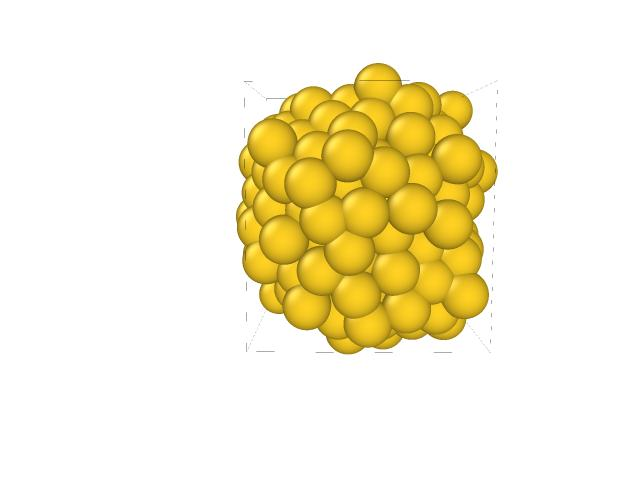
\includegraphics[trim={1.8cm 1.8cm 2.2cm 1cm},clip]{img/sim3.jpg}}
	\end{minipage}
	\caption{OVITO visualization of a cubic lattice with Berendsen thermostat. Without thermostat, atoms vaporize even with the smallest time step.}
	\label{fig:first_simulation_ovito}
\end{figure*}


I create a cube of atoms of width 4 for this experiment, Fig.~\ref{fig:first_simulation_ovito}

Choosing target temperature: 0.05 --- visualization shows that the atoms are pushed apart into infinity in small groups; 0.005 --- no vaporization.

Choosing Berendsen relaxation time: for the whole simulation, \(1000\Delta t\) is required to keep the atoms from evaporating; initial stronger relaxation didn't make a difference.

Testing the Berendsen implementation is very simple, because it modifies the speed of each atom separately, so it's enough to test the behaviour on just one atom. I tested that the temperature should exponentially approach the desired value, and in case the relaxation time is equal to \(\Delta t\), it should change instantly.

{\bf Implementation} --- src/lattice.cpp, src/lattice.h, src/thermostat.cpp, src/thermostat.h, tests/test\_thermostat.cpp milestones/05/main.cpp

\subsection*{Neighbor list}

\begin{figure*}[htb]
	\centering
	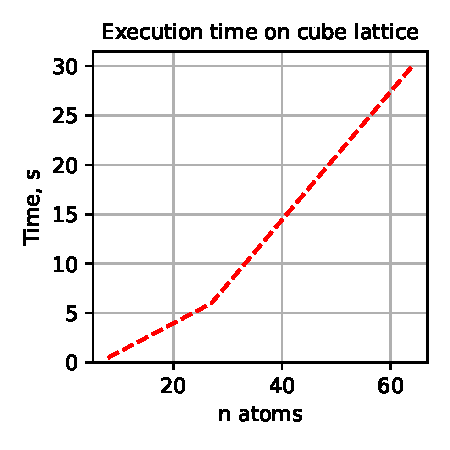
\includegraphics[width=.3\linewidth]{img/fig_pairwise.pdf}
	\caption{Without cutoff, time scales quadratically with number of atoms.}
	\label{fig:berendsen_time_pair}
\end{figure*}

\begin{figure*}[htb]
	\centering
	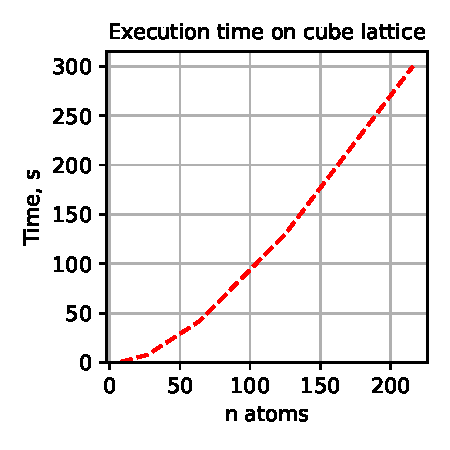
\includegraphics[width=.3\linewidth]{img/fig_neighbor.pdf}
	\caption{With cutoff, time scales linearly with number of atoms.}
	\label{fig:berendsen_time_neighbor}
\end{figure*}

The provided implementation of neighbor lists is used. Cutoff radius is \( 4 \sigma \) to allow speedup, but not miss important interactions. Execution time on clusters of different sizes is compared in Fig.~\ref{fig:berendsen_time_pair} and Fig.~\ref{fig:berendsen_time_neighbor}. Number of atoms: $2^3=8, 3^3=27, 4^3=64, 5^3=125$.

{\bf Implementation} --- src/neighbors.cpp, src/neighbors.h, tests/test\_neighbors.cpp, src/lj.cpp, src/lj.h, tests/test\_thermostat.cpp milestones/06/main.cpp

Run: \verb|cd buildDir/milestones/06; time ./milestone06|

\verb|lj_direct_summation|
\verb|lj_neighbor_list|
\verb|optimization level 3|

\begin{itemize}
	\item Outputs are generated in \verb|buildDir/milestones/05|
	\item Plot with \verb|plot/time_lineplot.ipynb|
\end{itemize}

\subsection*{Heating experiment}

\textcolor{red}{\large\bf At this point I found that total energy was not conserved because I recomputed forces after 2 Verlet step!}

{\bf Equilibration} with Berendsen thermostat is done for the first 100 fs with $\tau_T$ = 100 fs and target temperature 300 K = 27 C.

With correct force recomputation, even a large time step $\Delta t=10$ fs causes total energy drift no more than 1 eV in 100 000 fs (without thermostat and heat deposition), we can safely use it for this simulation. Before the error was fixed, it drifted no matter which $\Delta t$ I chose. Now I disable the thermostat after equilibration for fair energy measurements. Smaller $\Delta t = 1$ fs showed similar results. The intuition for choosing the time step is, that it must be much smaller than oscillation period of an atom. The gold atoms have large mass thus a large step is acceptable.

One oscillation takes around 1000 fs.

TODO Small cluster total = 100 000 fs, step = 10 fs, deposit = 4000 fs, delta Q = 20 eV. Big cluster delta Q = 100 eV. Whisker delta Q = 200 eV.

\subsubsection*{Adding heat}

To add a fixed amount of energy $Q$ we scale the velocities by $\lambda$:

\[
\begin{aligned}
	E_k &= \frac{1}{2} \sum_i m v_i^2 \\
	E_k + Q &= \frac{1}{2} \sum_i m (\lambda v_i)^2 = \lambda^2 \frac{1}{2} \sum_i m v_i^2 \\
	E_k + Q &= \lambda^2 E_k \\
	\lambda^2 &= 1 + \frac{Q}{E_k} \\
\end{aligned}
\]

{\centering\framed{ \( \lambda = \sqrt{1 + \frac{Q}{E_k}} \) }\\}

Latent heat is the energy to transform from solid to liquid state. During melting the temperature stays the same, but potential energy increases. Heat capacity is the coefficient $dE/dT$ of linear relation between $E_{tot}$ and $T$ (without thermostat it actually becomes linear).

I simulated the Makay-923 and Makay-3871 Makay clusters, introduced in \cite{MakayOriginal} and implemented by Dr Lars Pastewka in \cite{MakayPastewka} and generated Whisker-6950 using the \verb|make_whisker.py| script.
As the simulation doesn't have truly constant melting temperature, I took the middle point between linear regions on the energy-temperature plot (Fig.~\ref{fig:heat-makay1},~\ref{fig:heat-makay2},~\ref{fig:heat-whisker}). To measure the heat capacity coefficient I take two faraway points on the energy-temperature plot and compute $(E_2-E_1)/(T_2-T_1)$. To measure latent heat I extrapolate the lines for solid phase and liquid phase to the assumed melting point and take the difference in energies (Fig.~\ref{fig:heat-estimated}).

\begin{figure*}[h!]
	\centering
	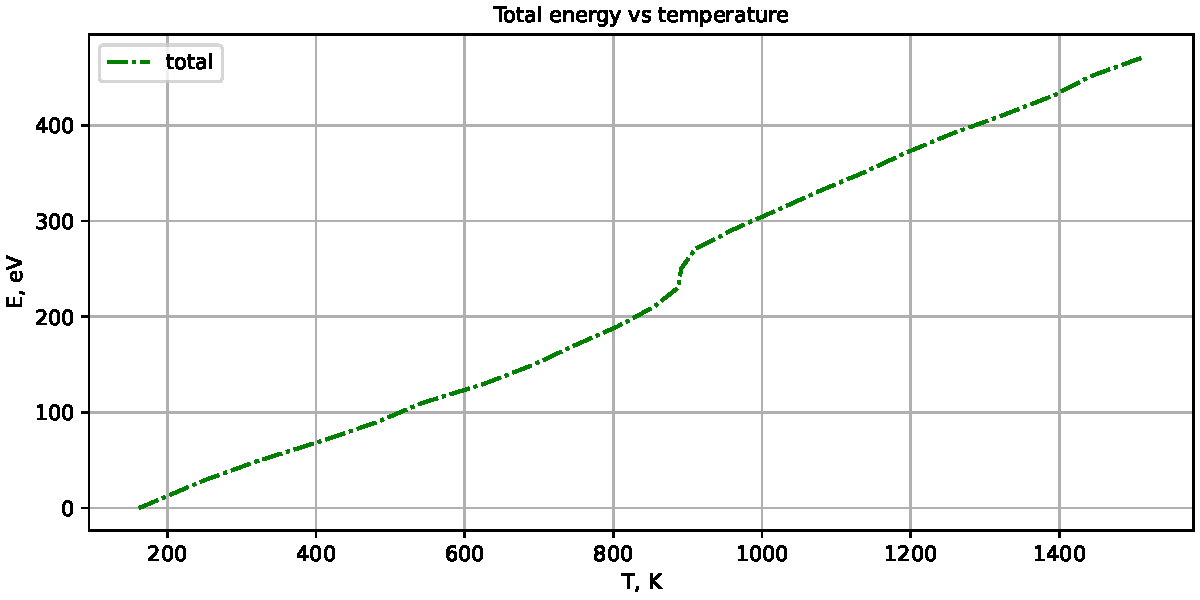
\includegraphics[width=.8\linewidth]{img/milestone07-small.pdf}
	\caption{Total energy (eV) vs temperature (K) for Makay-923.}
	\label{fig:heat-makay1}
\end{figure*}

\begin{figure*}[h!]
	\centering
	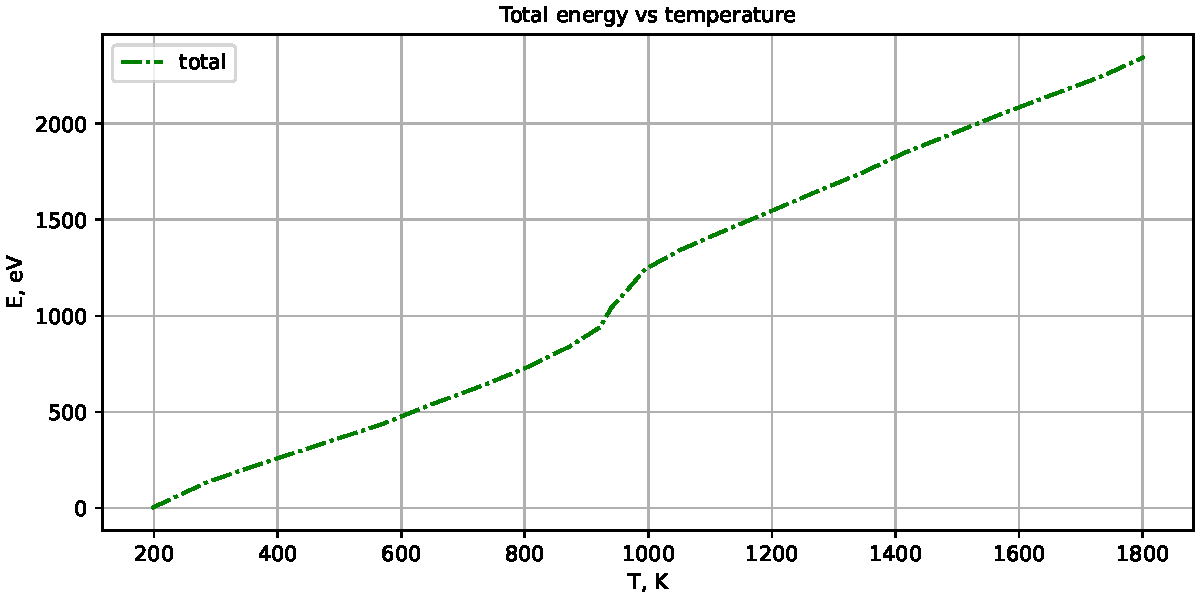
\includegraphics[width=.8\linewidth]{img/milestone07-large.pdf}
	\caption{Total energy (eV) vs temperature (K) for Makay-3871.}
	\label{fig:heat-makay2}
\end{figure*}

\begin{figure*}[h!]
	\centering
	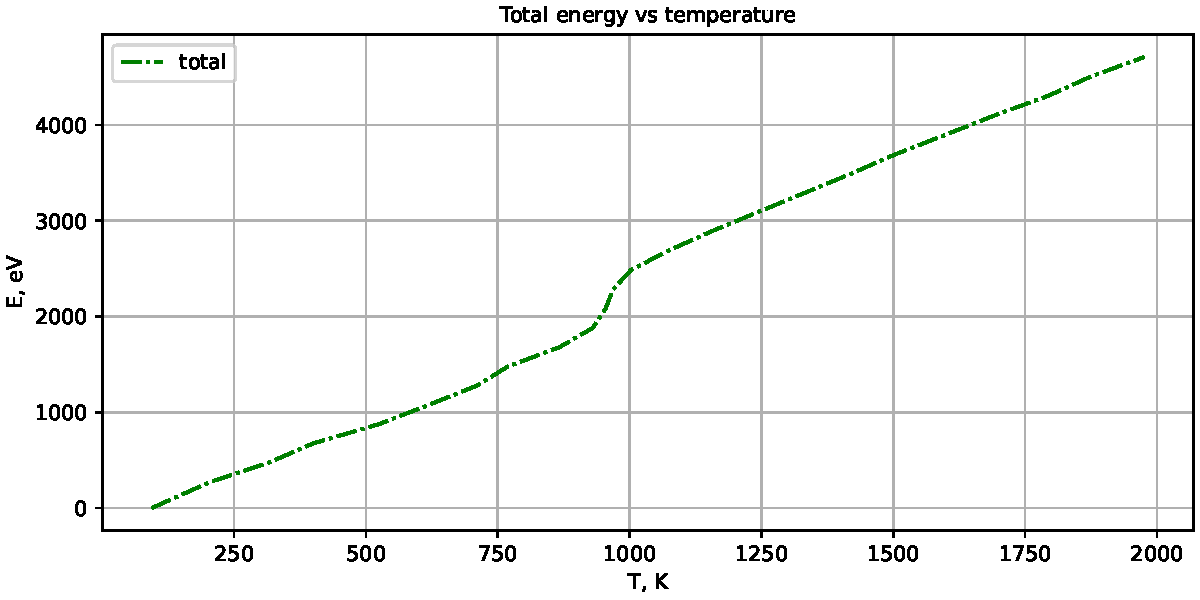
\includegraphics[width=.8\linewidth]{img/milestone07-whisker.pdf}
	\caption{Total energy (eV) vs temperature (K) for Whisker-6950.}
	\label{fig:heat-whisker}
\end{figure*}

\begin{figure*}[h!]
	\centering
	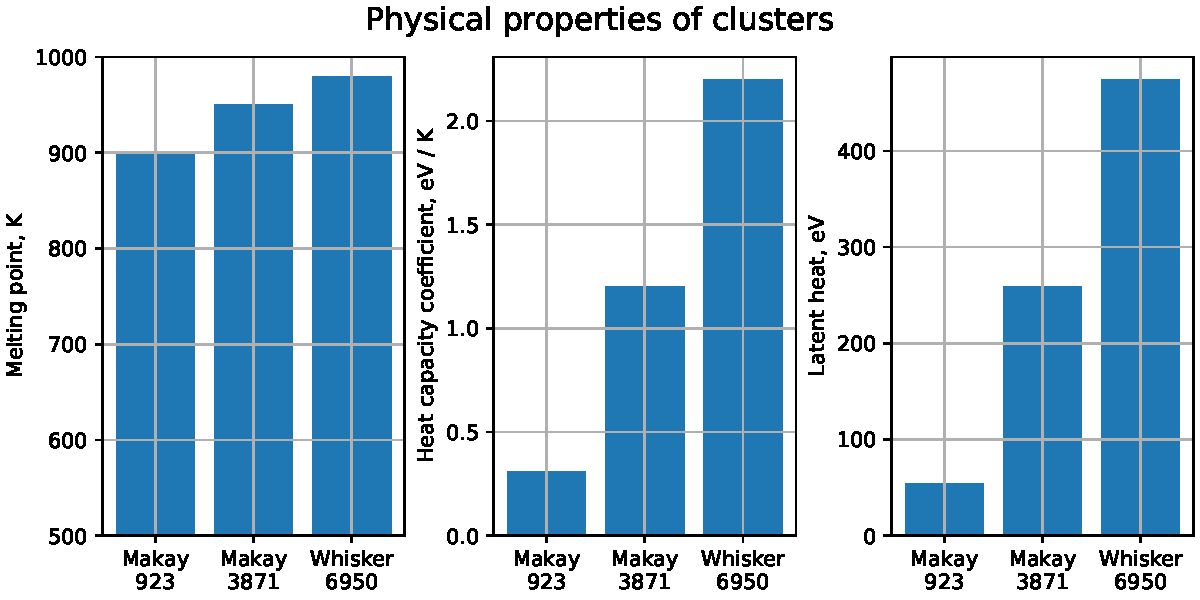
\includegraphics[width=.9\linewidth]{img/milestone07-bar.pdf}
	\caption{Estimated Melting point (K), Heat capacity coefficient, Latent heat (eV) for each cluster.}
	\label{fig:heat-estimated}
\end{figure*}

\newpage

{\bf Implementation} --- src/ducastelle.h, src/ducastelle.cpp, milestones/07/main.cpp

\begin{itemize}
	\item Outputs are generated in \verb|buildDir/milestones/07|
	\item Plot with \verb|plot/milestone07.ipynb|
\end{itemize}

\newpage

\subsection*{Parallelization}

Atoms on the domain edge disappear. Solution: add offset to positions.

I used the gold cluster Mackay-3871. With $\Delta t$ = 10 fs, total energy fluctuates no more than 0.5 eV in 10 000 fs, simulation for 100 000 fs didn't show larger fluctuation. Also, the temperature plot shows that atom oscillation has a period of around 1000 fs, it confirms that our step size is reasonable.

Compile, domain (1, 2, 2),
\verb|mpirun -n 4 --oversubscribe ./milestone08|

\begin{itemize}
	\item Outputs are generated in \verb|buildDir/milestones/08|
	\item Plot with \verb|plot/milestone08.ipynb|
\end{itemize}

\begin{figure*}[h!]
	\centering
	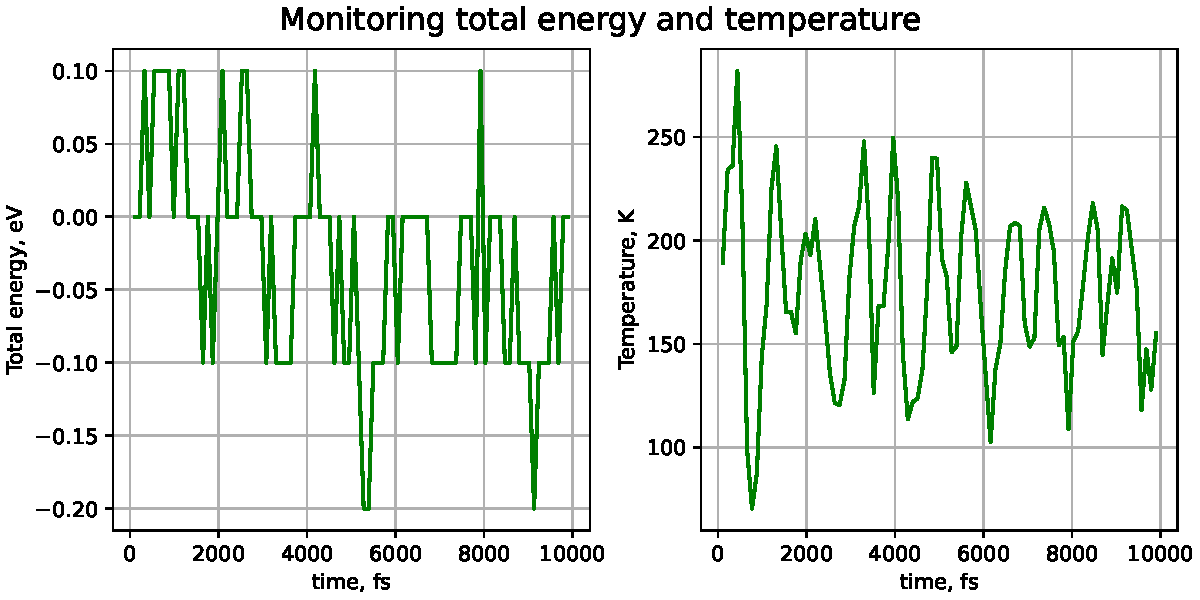
\includegraphics[width=.9\linewidth]{img/milestone08-1proc.pdf}
	\caption{Parallelized with 1 process.}
	\label{fig:parallel-1}
\end{figure*}

\begin{figure*}[h!]
	\centering
	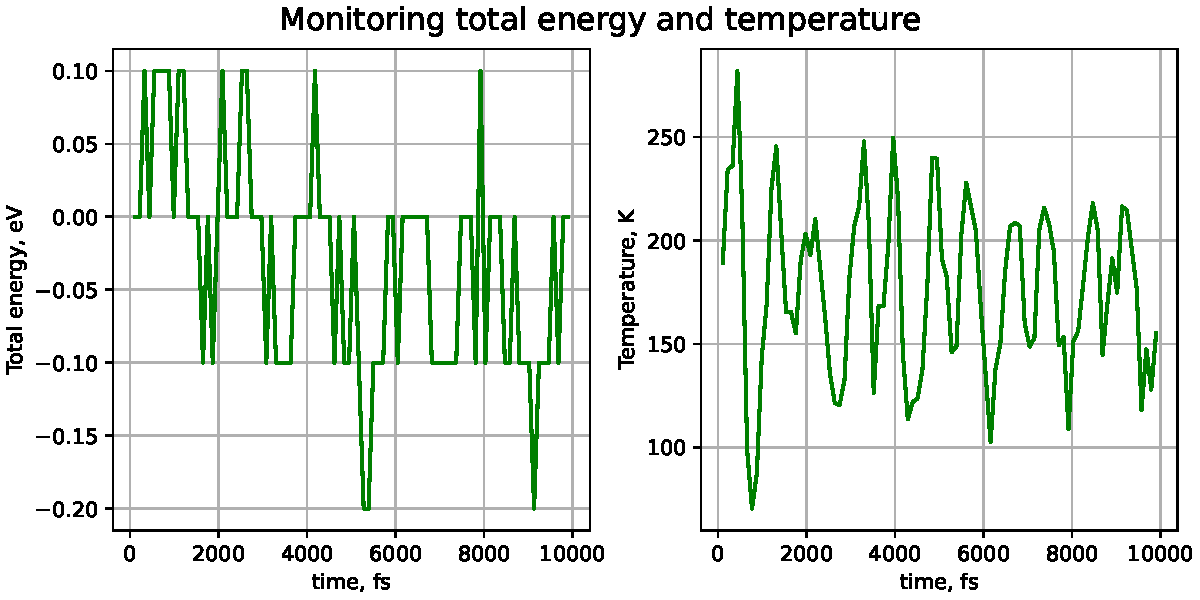
\includegraphics[width=.9\linewidth]{img/milestone08-4proc.pdf}
	\caption{Parallelized with 4 processes.}
	\label{fig:parallel-2}
\end{figure*}

\begin{figure*}[h!]
	\centering
	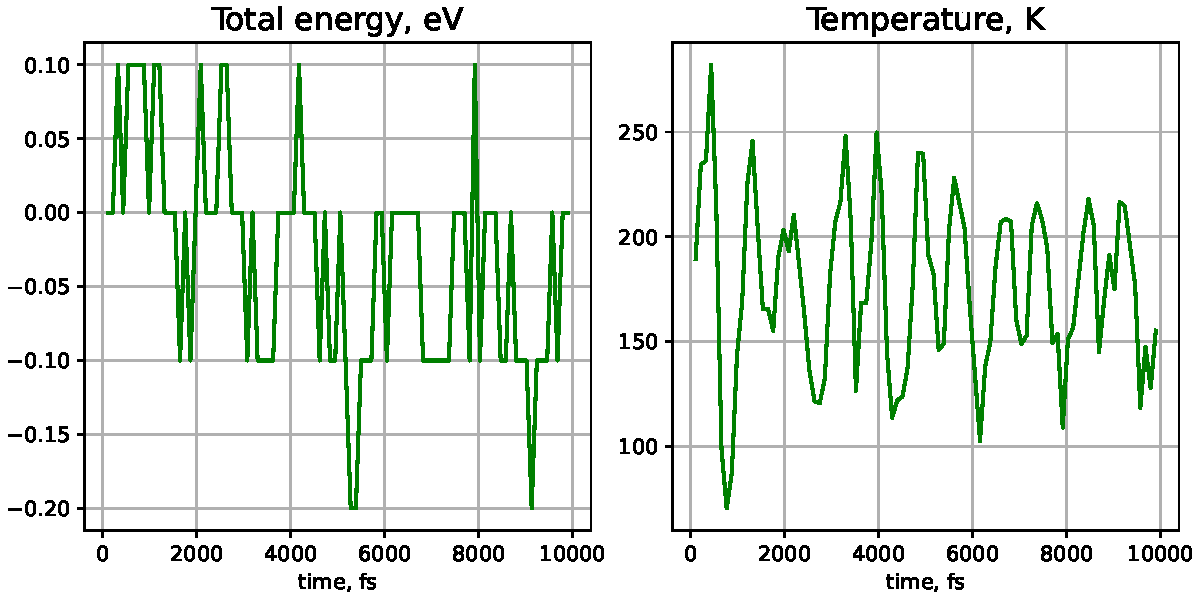
\includegraphics[width=.9\linewidth]{img/milestone08-8proc.pdf}
	\caption{Parallelized with 8 processes.}
	\label{fig:parallel-3}
\end{figure*}

\clearpage % works for figures too!

\section{Conclusion}
\label{conclusion}

I should have planned to complete the project much earlier. The MPI part is well known, but it takes a lot of time to adapt the simulation code and debug.

\newpage
{\small
	\bibliographystyle{plain}
	\bibliography{egbib}
}

\end{document}
